\appendix
\chapter{Statistics}
\section{Statistics}
% remove comment if you wish to add Appendix to contentsline.
%\addcontentsline{toc}{chapter}{Appendix A: How to download ERA5 data}
%%%% MEAN
\begin{figure}[ht]
    \centering
    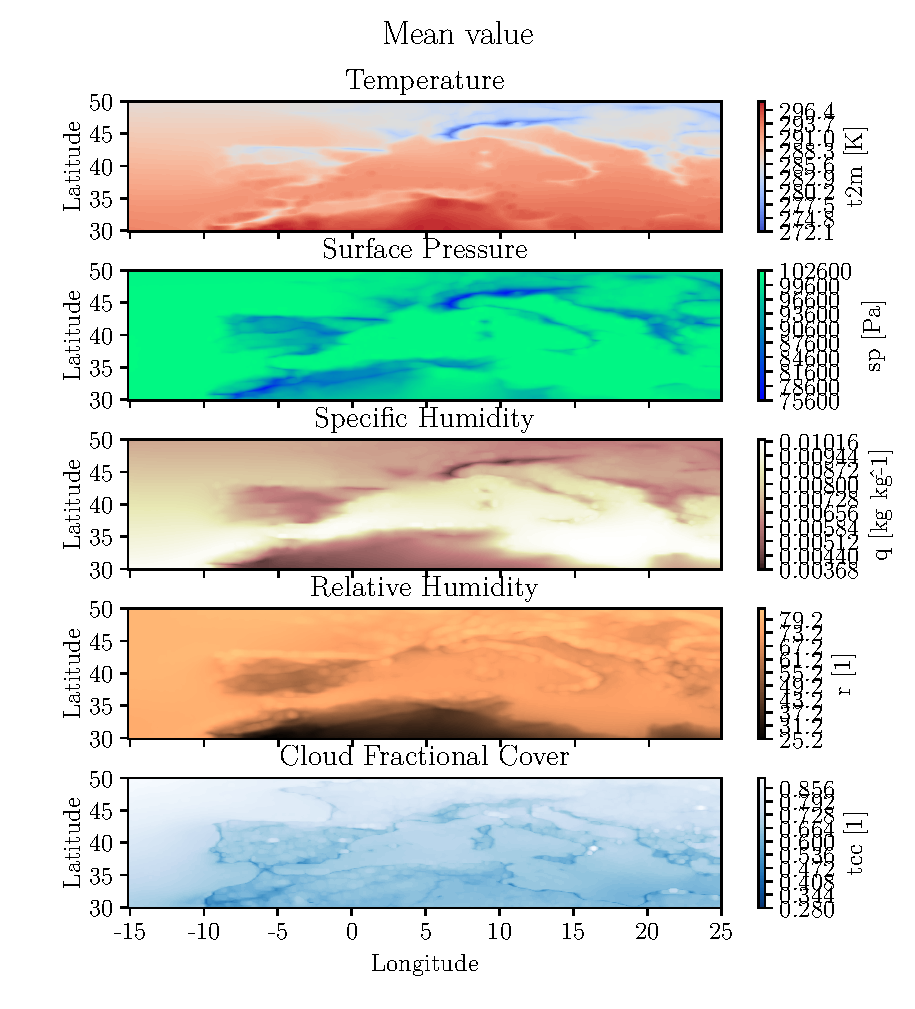
\includegraphics{python_figs/contourplot_all_variables_mean.pdf}
    \caption{Contour plot showing the local (pixel) mean of all variables.}
    \label{fig:contour_mean_all_vars}
\end{figure}




\section{Alternative 1 - all statistical property for one variable}

%%% ALL LOCAL STATISTICS FOR VARIABLES 
%% TEMPERATURE
\begin{figure}[ht]
    \centering
    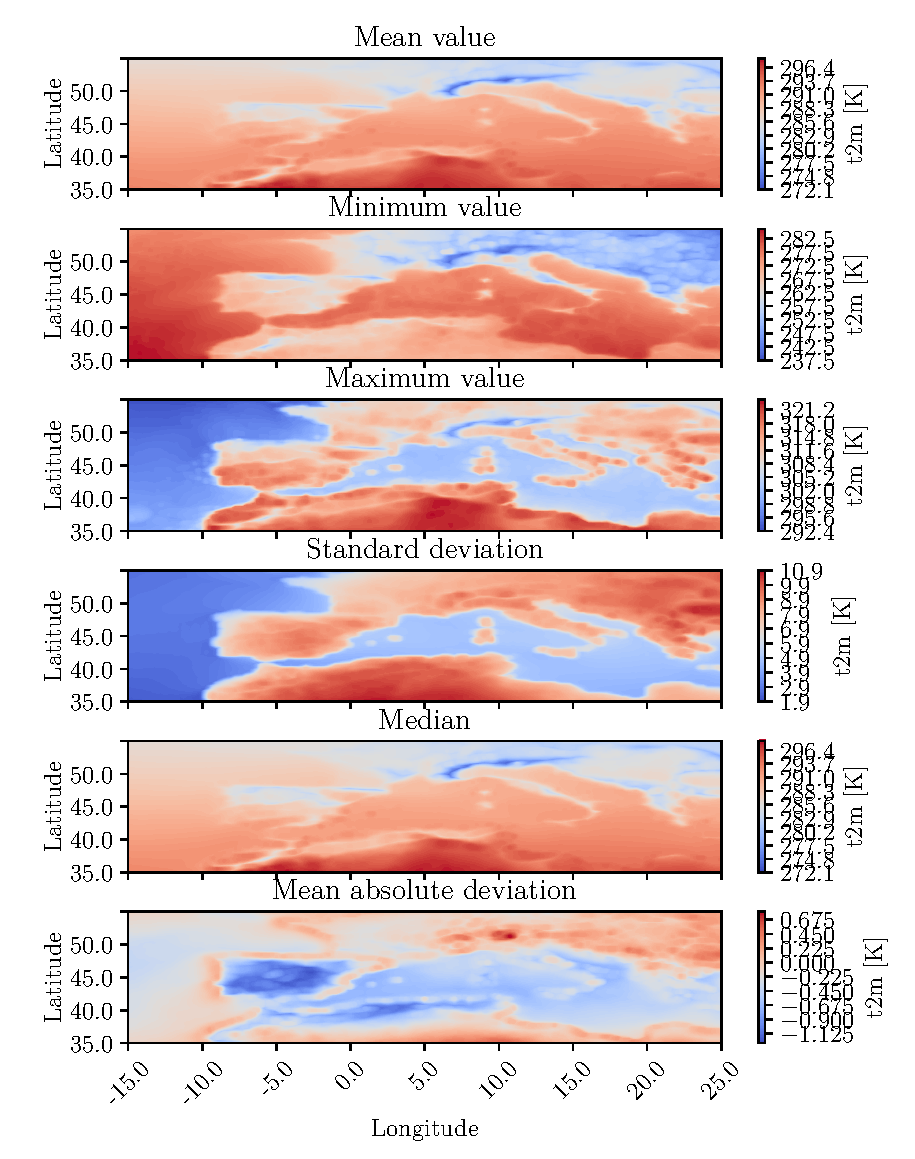
\includegraphics{python_figs/all_stat_variable_t2m.pdf}
    \caption{Contour plot showing the local (pixel) statistics for temperature.}
    \label{fig:all_stats_t2m}
\end{figure}

%% SURFACE PRESSURE 
\begin{figure}[ht]
    \centering
    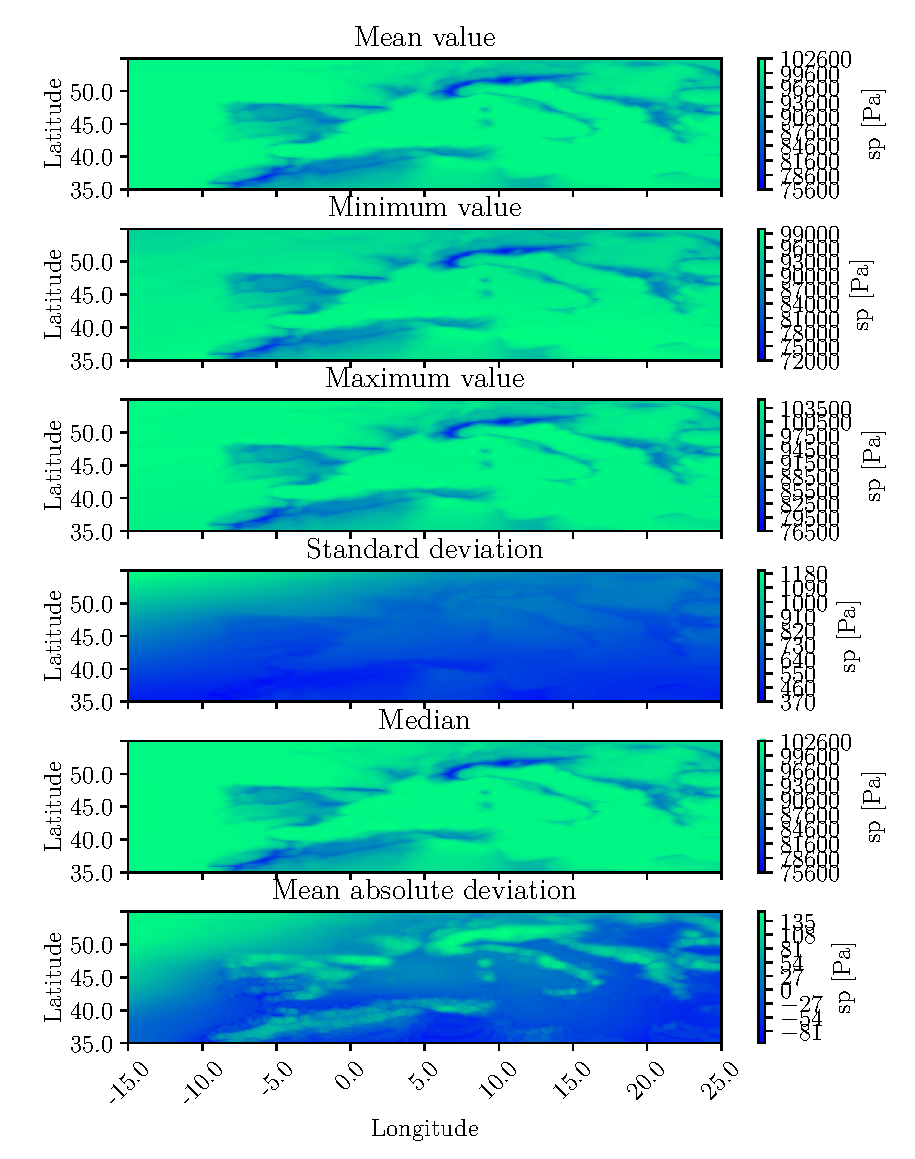
\includegraphics{python_figs/all_stat_variable_sp.pdf}
    \caption{Contour plot showing the local (pixel) statistics for surface pressure.}
    \label{fig:all_stats_sp}
\end{figure}

%% RELATIVE HUMIDITY 
\begin{figure}[ht]
    \centering
    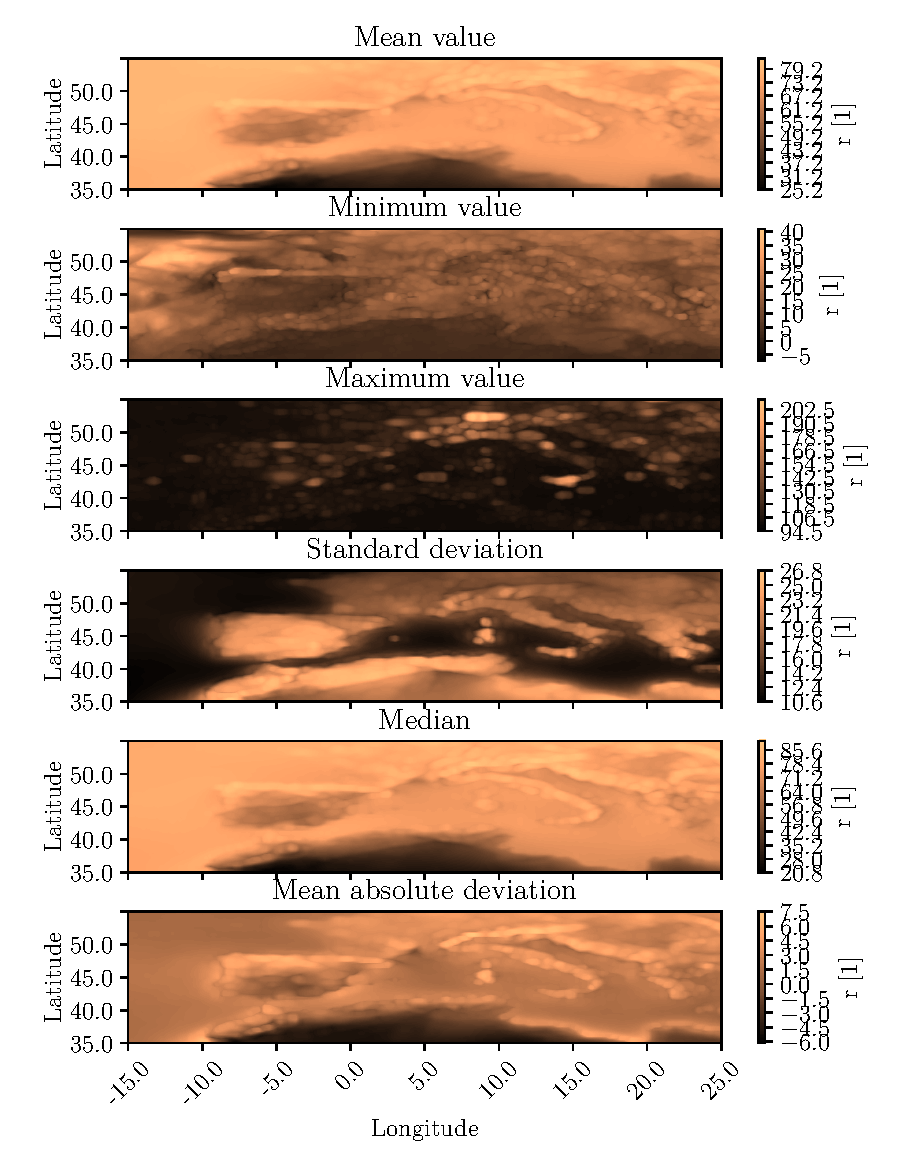
\includegraphics{python_figs/all_stat_variable_r.pdf}
    \caption{Contour plot showing the local (pixel) statistics for relative humidity.}
    \label{fig:all_stats_r}
\end{figure}


%% SPECIFIC HUMIDITY 
\begin{figure}[ht]
    \centering
    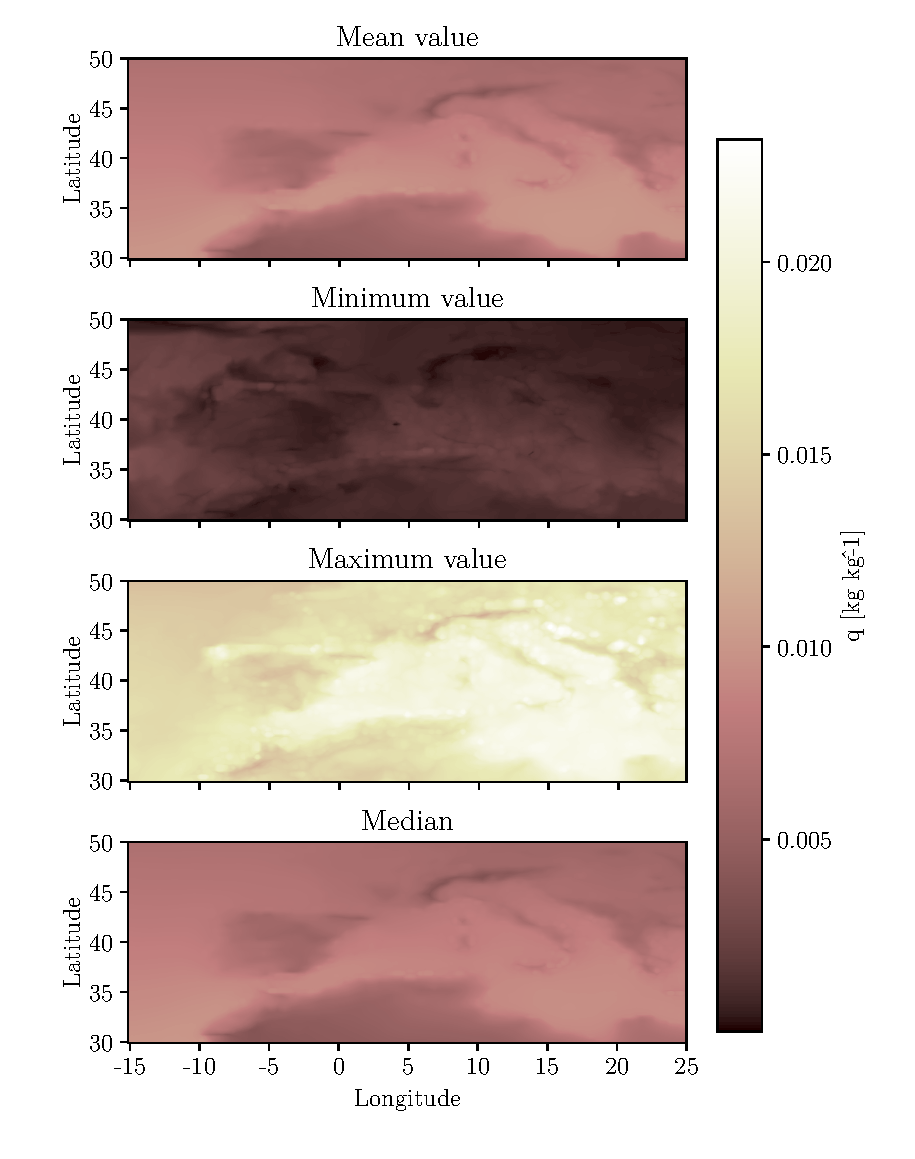
\includegraphics{python_figs/all_stat_variable_q.pdf}
    \caption{Contour plot showing the local (pixel) statistics for spesific humidity.}
    \label{fig:all_stats_q}
\end{figure}


\begin{figure}
    \centering
    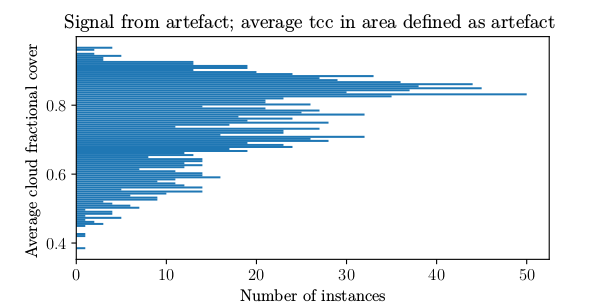
\includegraphics{python_figs/signal_artefact.png}
    \caption{Occurence of artefact, keep in mind that is not made any effort to distinguish this from when the entire area has cloud cover, this could be done by the ratio of artefact signal to land or something else. }
    \label{fig:signal_artefact}
\end{figure}

%%%%%% CONTOUR PLOTS SHOWING 
%\subsection{Alternative 2 - sortert basert på statestikk }
%%%% STD
\begin{figure}[ht]
    \centering
    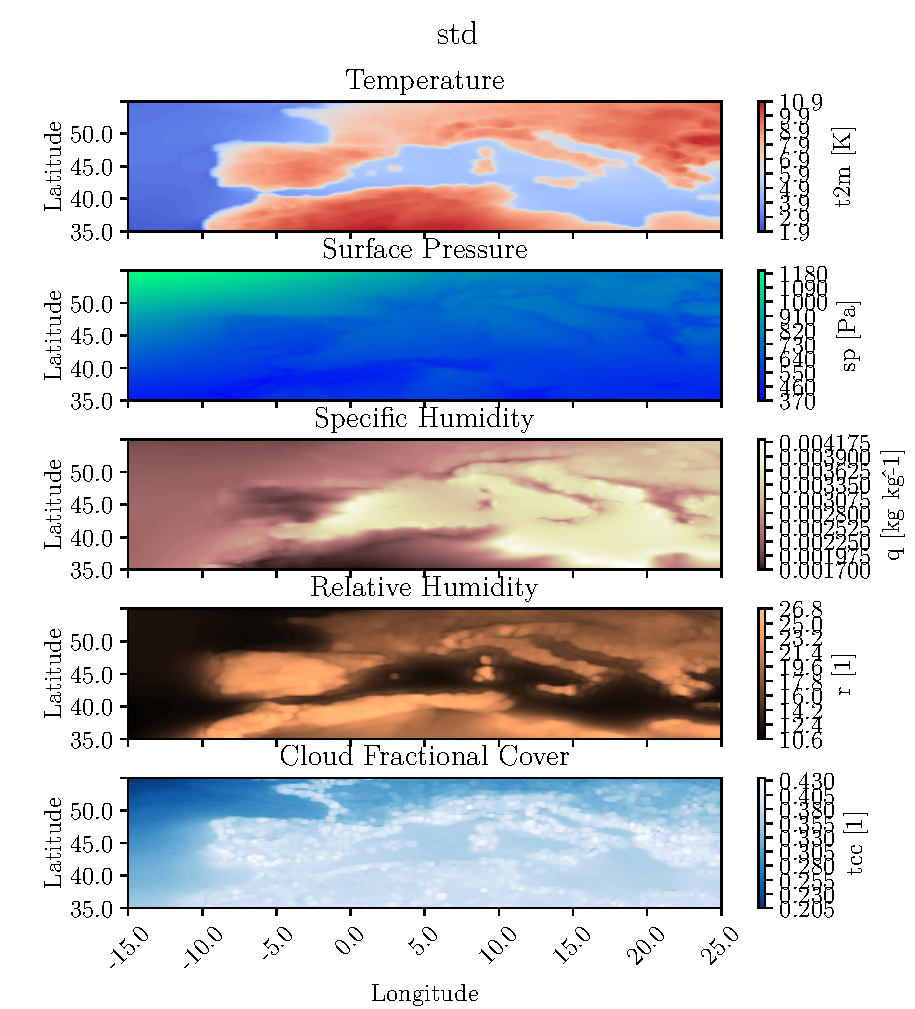
\includegraphics{python_figs/contourplot_all_variables_std.pdf}
    \caption{Contour plot showing the local (pixel) standard deviation of all variables.}
    \label{fig:contour_std_all_vars}
\end{figure}

%%%% MIN
\begin{figure}[ht]
    \centering
    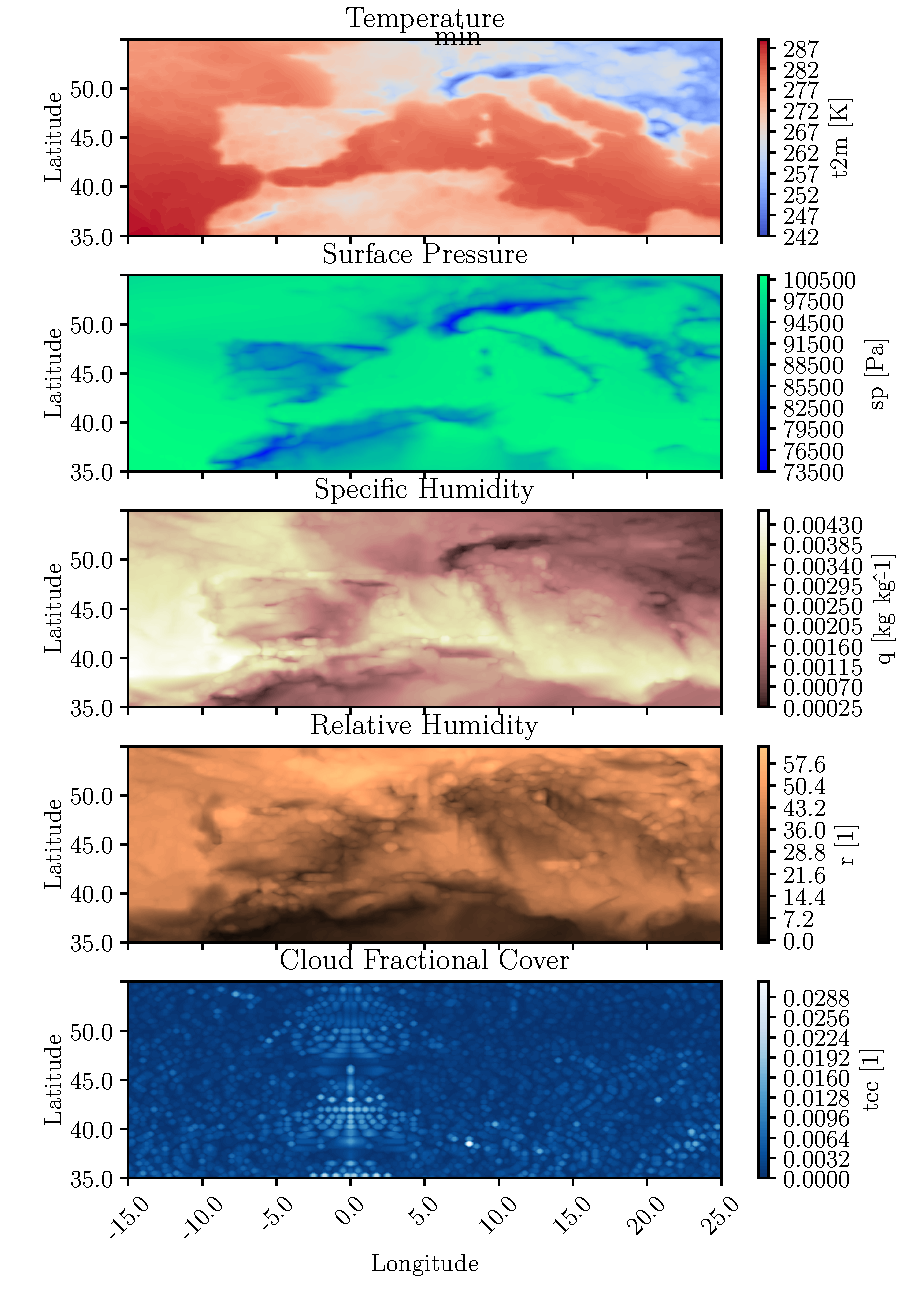
\includegraphics{python_figs/contourplot_all_variables_min.pdf}
    \caption{Contour plot showing the local (pixel) minimum of all variables.}
    \label{fig:contour_min_all_vars}
\end{figure}


%%%% MAX
\begin{figure}[ht]
    \centering
    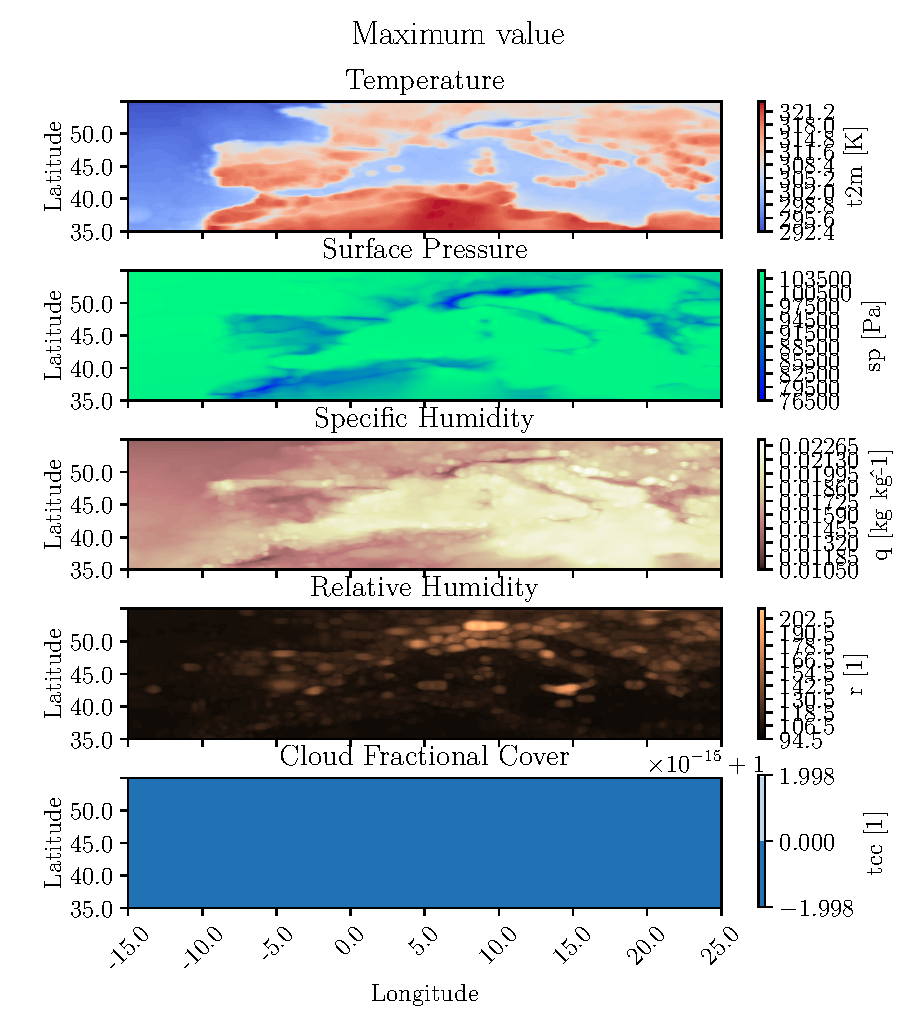
\includegraphics{python_figs/contourplot_all_variables_max.pdf}
    \caption{Contour plot showing the local (pixel) max of all variables.}
    \label{fig:contour_max_all_vars}
\end{figure}


%%%% MAD
\begin{figure}[ht]
    \centering
    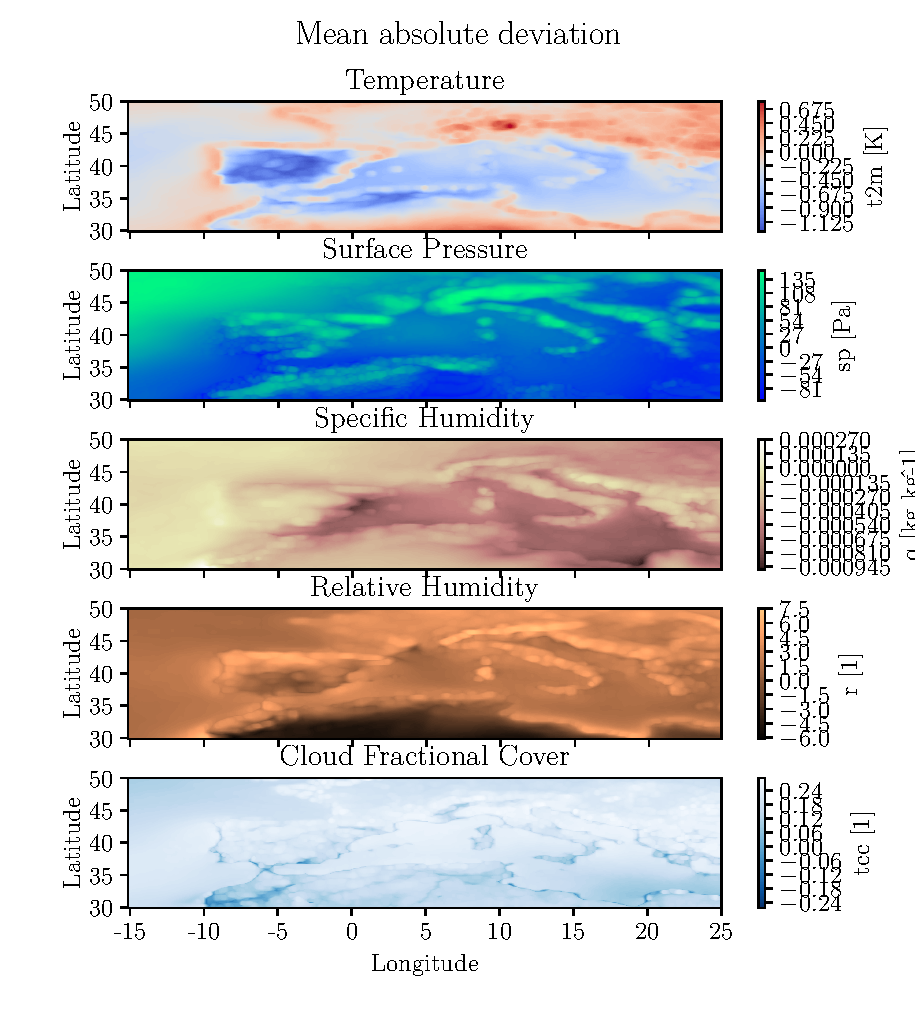
\includegraphics{python_figs/contourplot_all_variables_mad.pdf}
    \caption{NOT generated yet! Contour plot showing the local (pixel) mad of all variables.}
    \label{fig:contour_mad_all_vars}
\end{figure}


%%%% MEAN
\begin{figure}[ht]
    \centering
    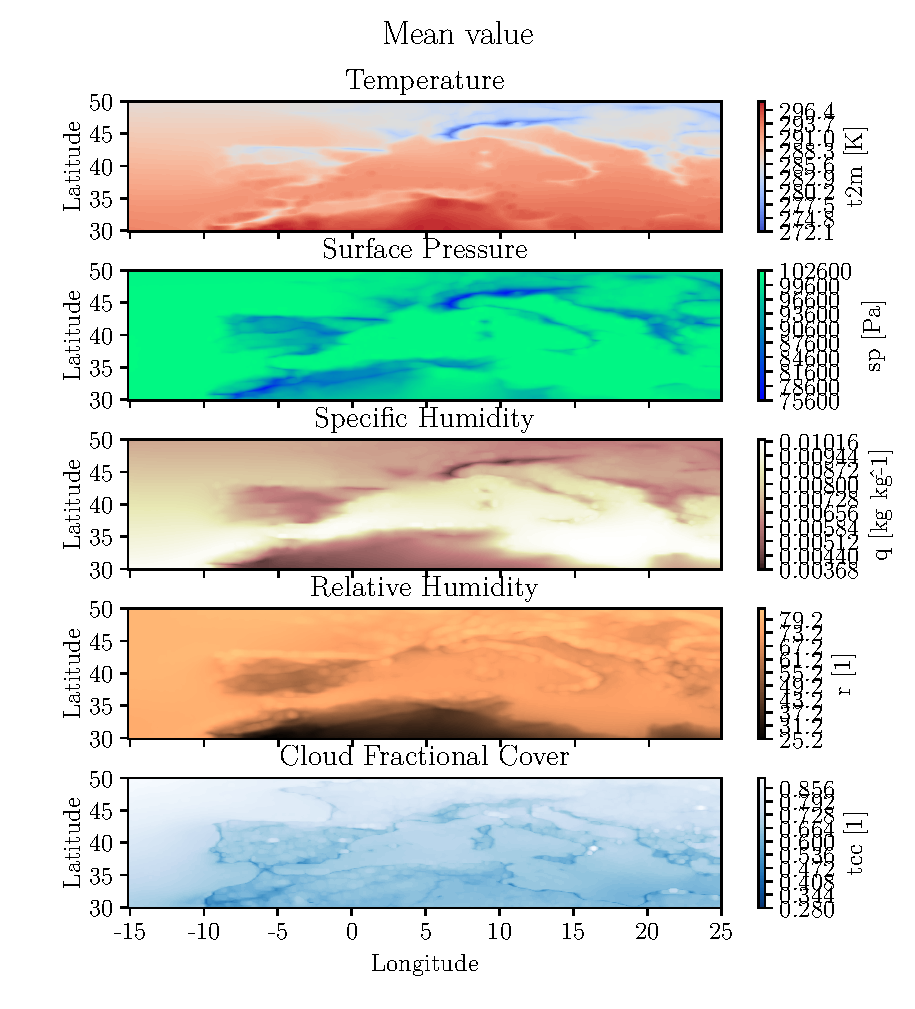
\includegraphics{python_figs/contourplot_all_variables_mean.pdf}
    \caption{Contour plot showing the local (pixel) mean of all variables.}
    \label{fig:contour_mean_all_vars}
\end{figure}


%%%% MEDIAN
\begin{figure}[ht]
    \centering
    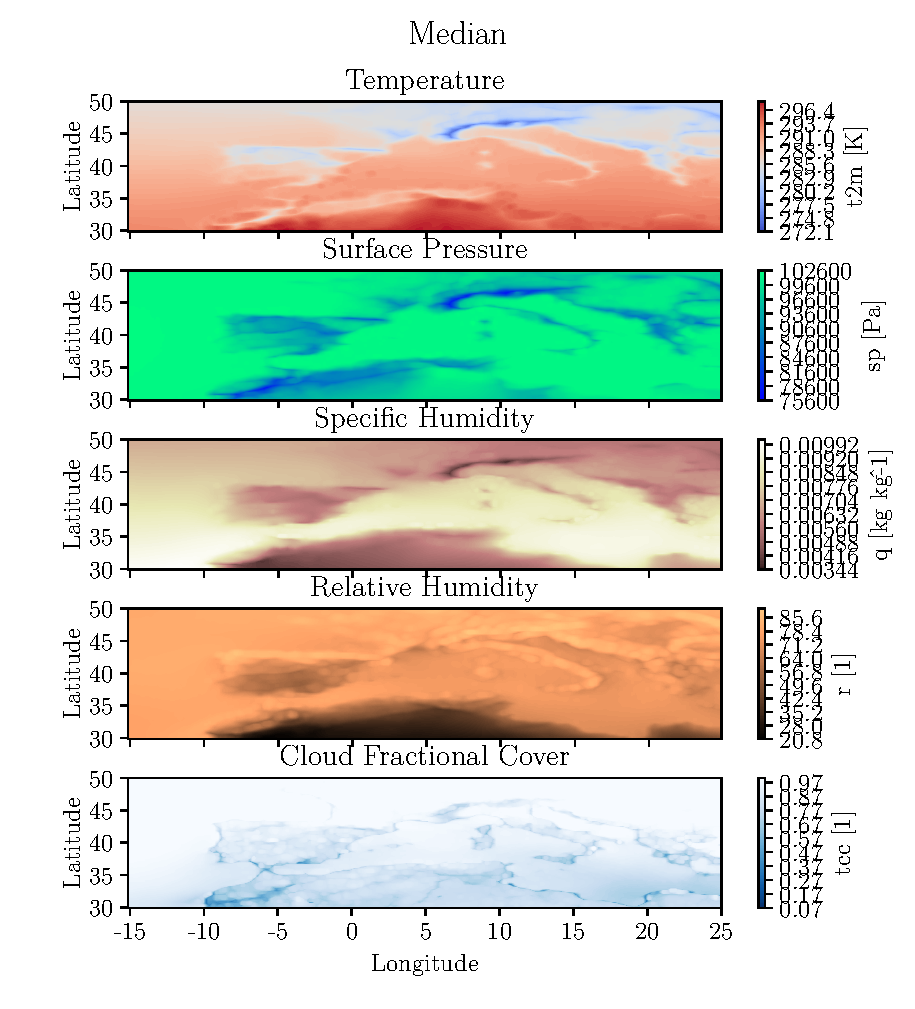
\includegraphics{python_figs/contourplot_all_variables_median.pdf}
    \caption{Contour plot showing the local (pixel) median of all variables.}
    \label{fig:contour_mean_all_vars}
\end{figure}


%%%%%%%%%%%%%%%%%%%%%%%%%%%5 seasonal statistics 

\cleardoublepage
\begin{figure}[ht]
    \centering
    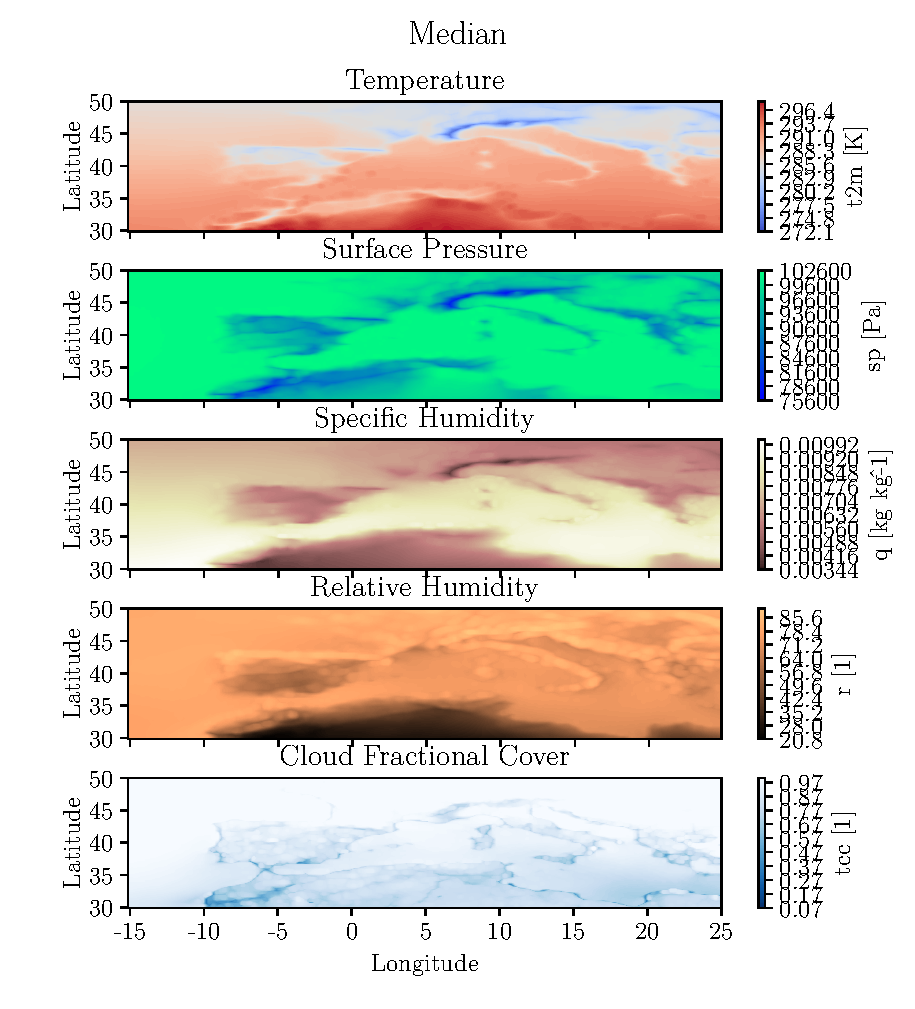
\includegraphics{python_figs/contourplot_all_variables_median.pdf}
    \caption{Contour plot showing the local (pixel) median of all variables.}
    \label{fig:contour_mean_all_vars}
\end{figure}

\chapter{Performance of other models}


%%%% TARGET PREDICITON HORIZONTAL
\begin{figure}[ht]
    \centering
    \includegraphics{python_figs/target_prediction_plot_horizonal.pdf}
    \caption{Comparison target and predicted cloud fractional cover.}
    \label{fig:target_predict_horizontal}
\end{figure}

%%%% TARGET PREDICITON HORIZONTAL
\begin{figure}[ht]
    \centering
    \includegraphics{python_figs/target_prediction_plot_vertical.pdf}
    \caption{Comparison target and predicted vertical cloud fractional cover.}
    \label{fig:target_predict_vertical}
\end{figure}

%%%% TARGET PREDICITON ERA5
\begin{figure}[ht]
    \centering
    \includegraphics{python_figs/target_prediction_era5_plot_horizonal.pdf}
    \caption{Comparison target, predicted and era5 horizontal cloud fractional cover.}
    \label{fig:target_predict_era5_vertical}
\end{figure}

%%%%%%%%%% Traditional AR model
%\begin{figure}[ht]
%    \centering
%    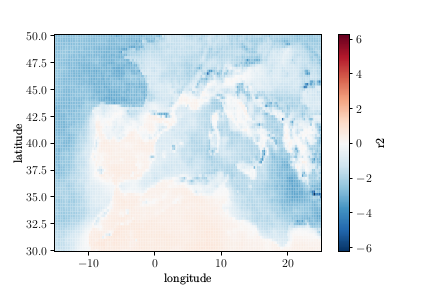
\includegraphics{python_figs/test_traditional_ar_r2.png}
%    \caption{Trained model traditional ar of order 2. Ove land it seems ok, over ocean and montain area seems difficult.}
%    \label{fig:traditional_ar_model_order_1}
%\end{figure}

%%%%%%%%%% Dummy model performance plot
%\begin{figure}[ht]
%    \centering
%    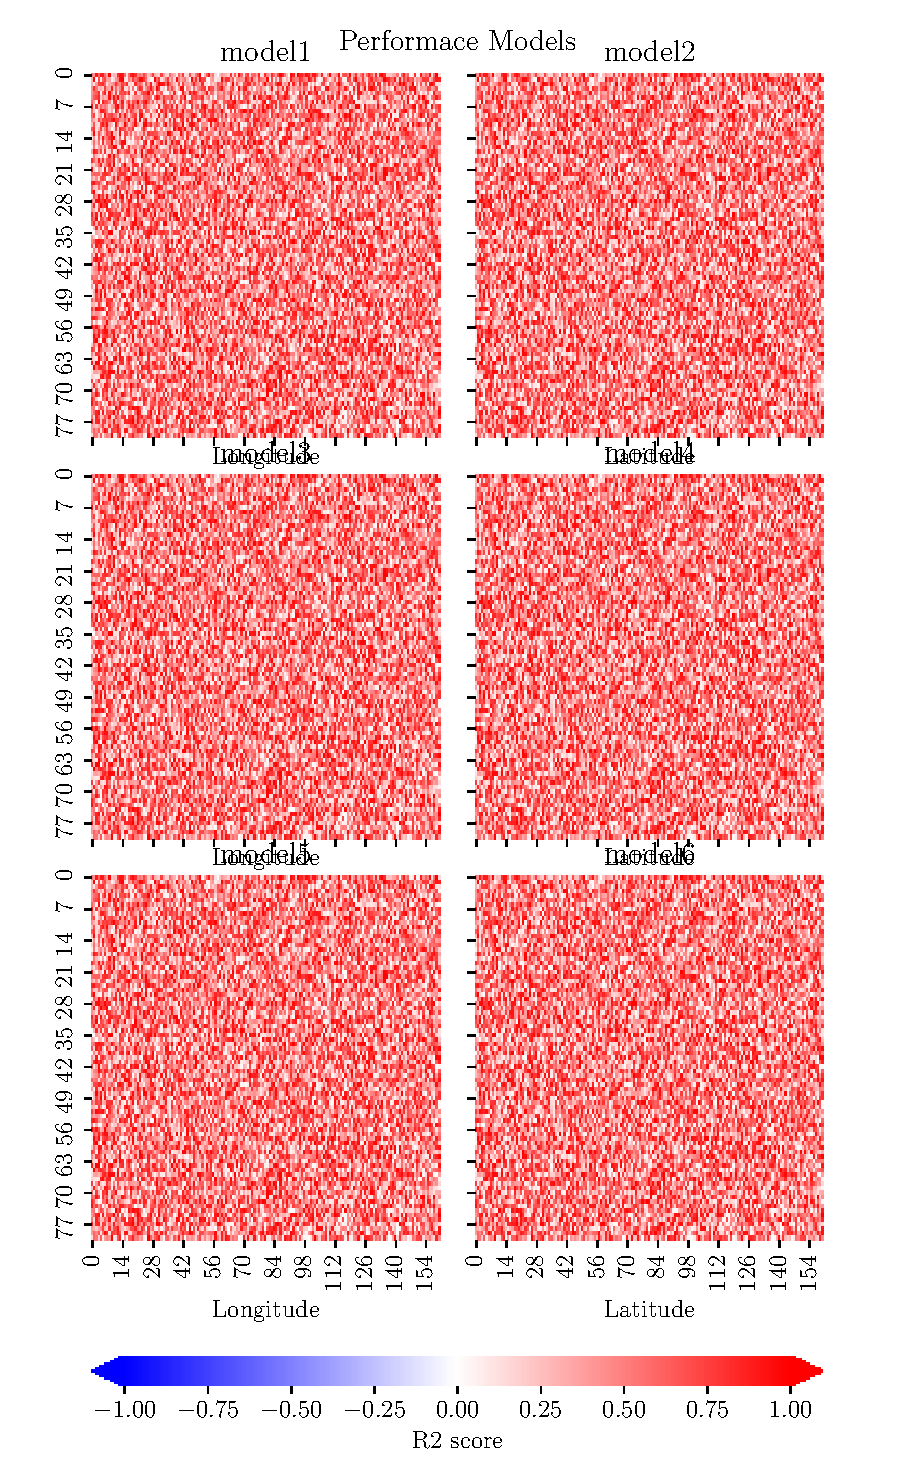
\includegraphics{python_figs/dummy_model_performace_plot.pdf}
%    \caption{Dummy performance plot.}
%    \label{fig:dummy_performace_plot}
%\end{figure}

%%%%%%%%%% Dummy model performance plot - CROSSVALIDATION
%\begin{figure}[ht]
%    \centering
%    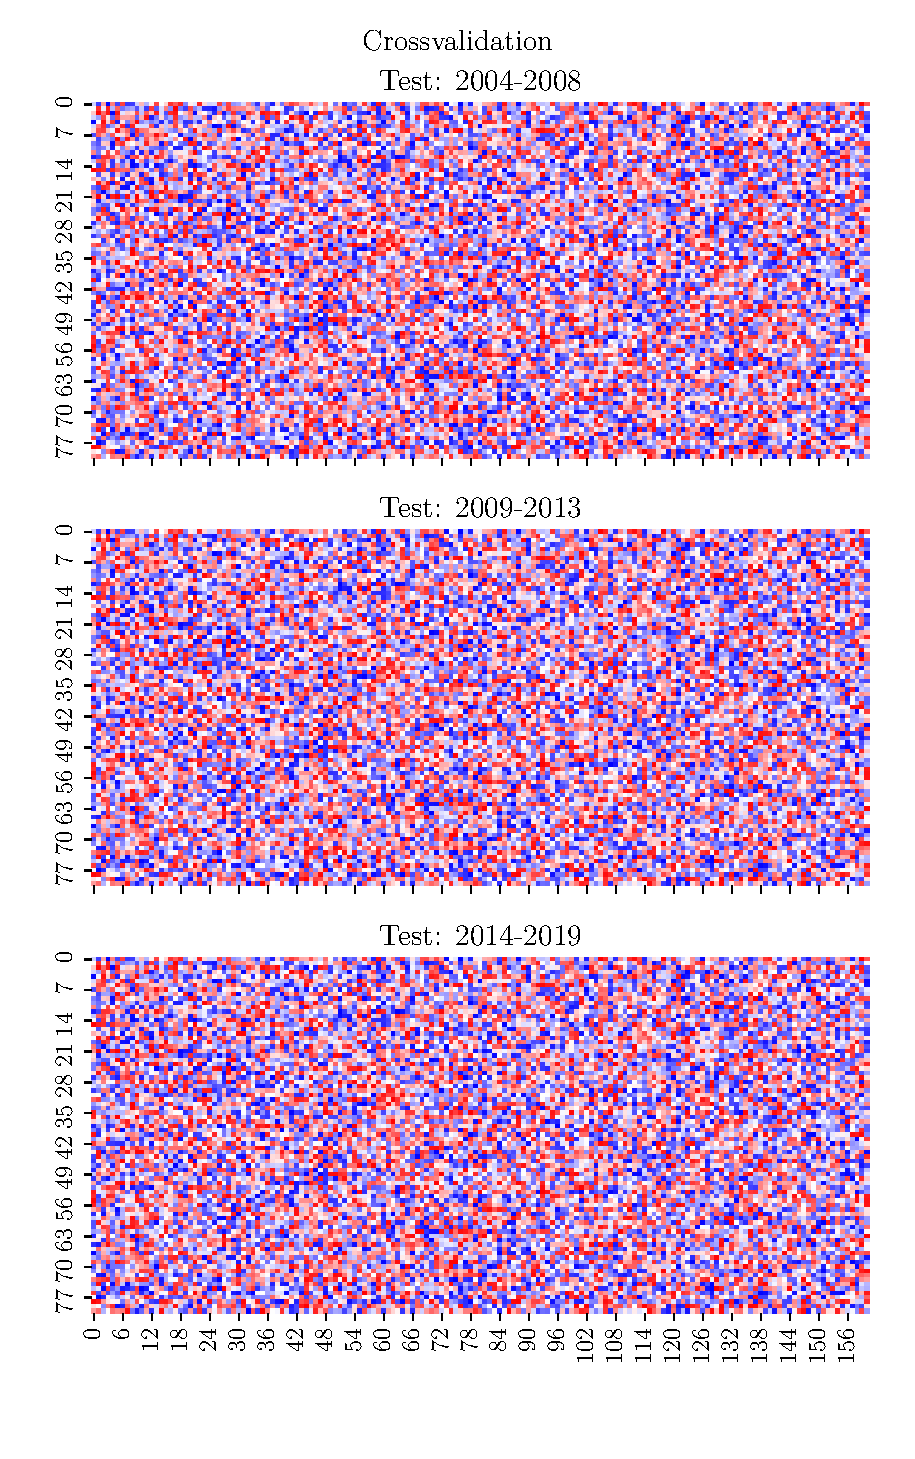
\includegraphics{python_figs/dummy_model_performace_cross_validation_plot.pdf}
%    \caption{Dummy performance plot - Crossvalidation edition.}
%    \label{fig:dummy_performace_plot_crossvalidation}
%\end{figure}

\cleardoublepage


\chapter{Time lapse cloud cover}

\begin{figure}[ht]
    \centering
    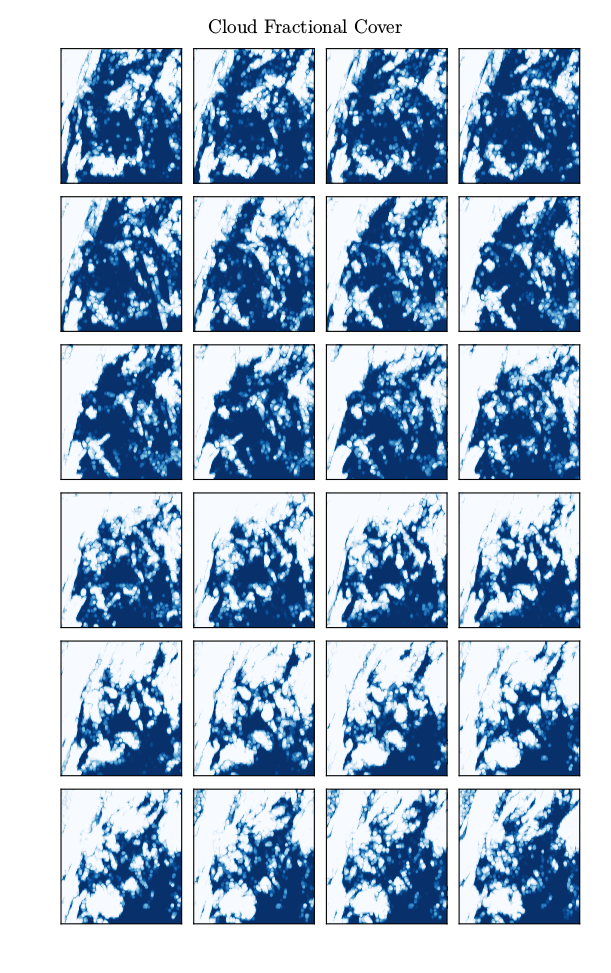
\includegraphics[scale=0.7]{python_figs/timelapse_cloud_cover_24hrs_from_2010-07-01.png}
    \caption{Time lapse photo, trying to detect the signal you would get from cloud cover within 24 hours.}
    \label{fig:time_lapse}
\end{figure}



\chapter{Study seasonal signals as temporal sequences - first week of every month in 2012}
%\addcontentsline{toc}{chapter}{Appendix D: Study 2012}

\begin{figure}[ht]
    \centering
    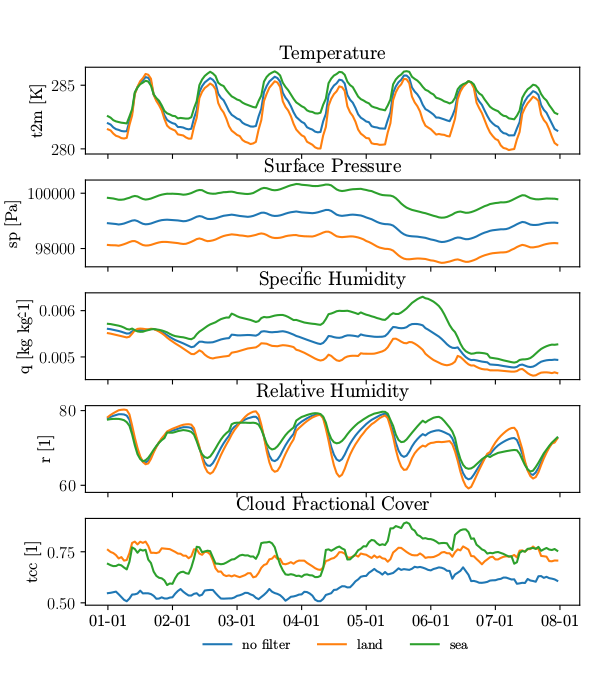
\includegraphics{python_figs/spatially_averaged_one_week_from_2012-01-01.png}
    \caption{Signal January 2012.}
    \label{fig:jan12}
\end{figure}

\begin{figure}[ht]
    \centering
    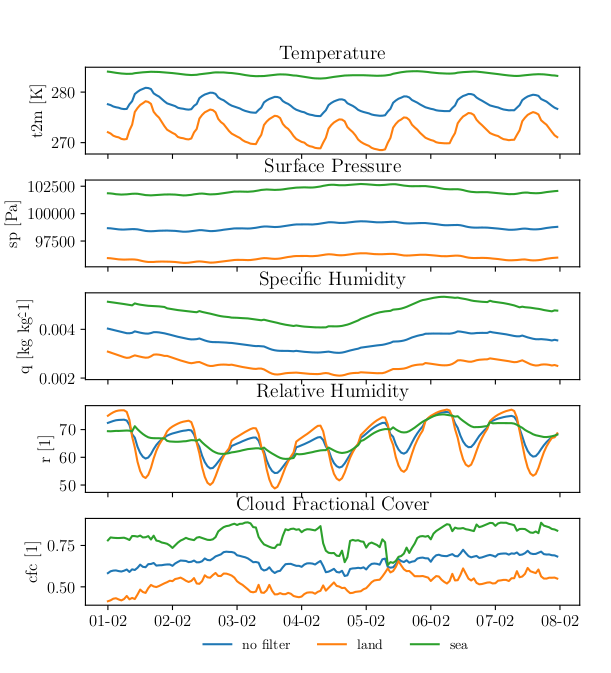
\includegraphics{python_figs/spatially_averaged_one_week_from_2012-02-01.png}
    \caption{Signal February 2012.}
    \label{fig:feb12}
\end{figure}

\begin{figure}[ht]
    \centering
    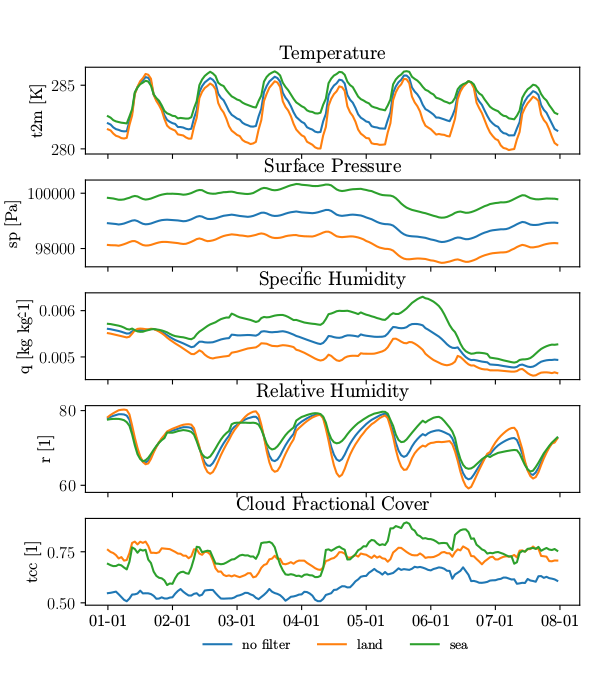
\includegraphics{python_figs/spatially_averaged_one_week_from_2012-01-01.png}
    \caption{Signal March 2012.}
    \label{fig:jan12}
\end{figure}
\begin{figure}[ht]
    \centering
    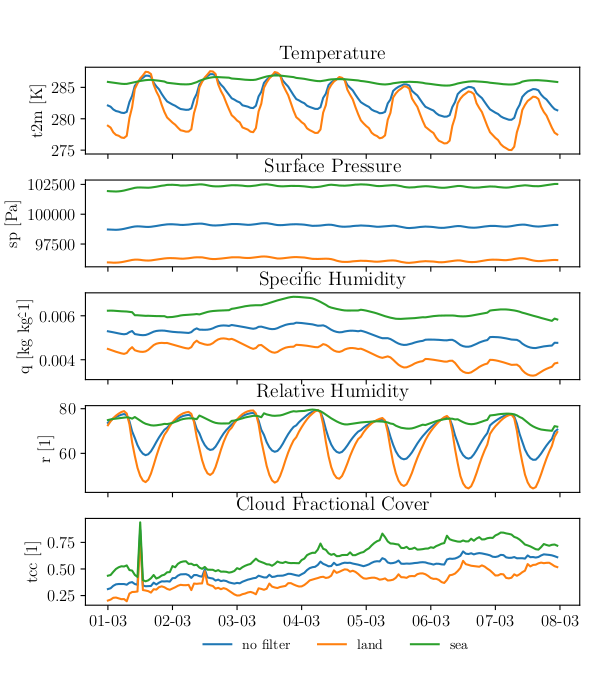
\includegraphics{python_figs/spatially_averaged_one_week_from_2012-03-01.png}
    \caption{Signal January 2012.}
    \label{fig:jan12}
\end{figure}
\begin{figure}[ht]
    \centering
    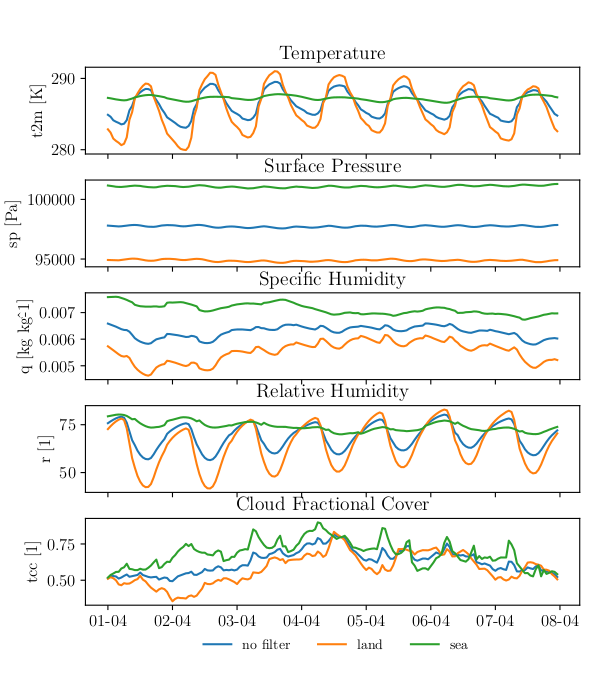
\includegraphics{python_figs/spatially_averaged_one_week_from_2012-04-01.png}
    \caption{Signal April 2012.}
    \label{fig:april12}
\end{figure}



\begin{figure}[ht]
    \centering
    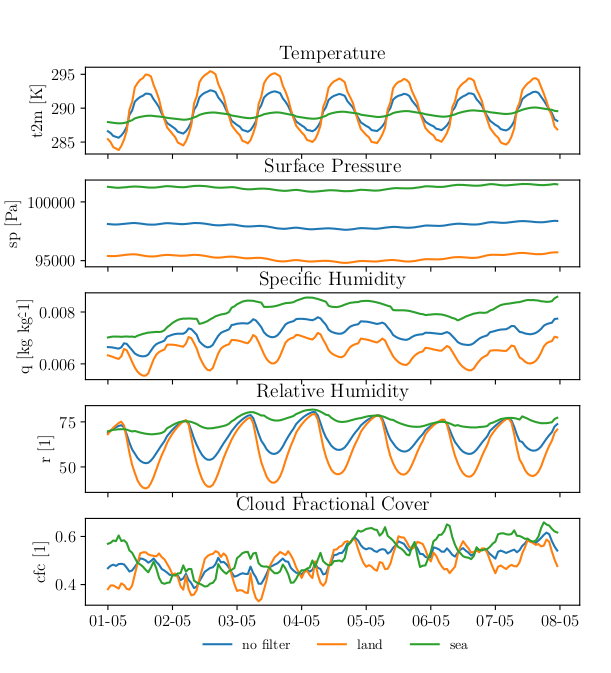
\includegraphics{python_figs/spatially_averaged_one_week_from_2012-05-01.png}
    \caption{Signal May 2012.}
    \label{fig:may12}
\end{figure}


\begin{figure}[ht]
    \centering
    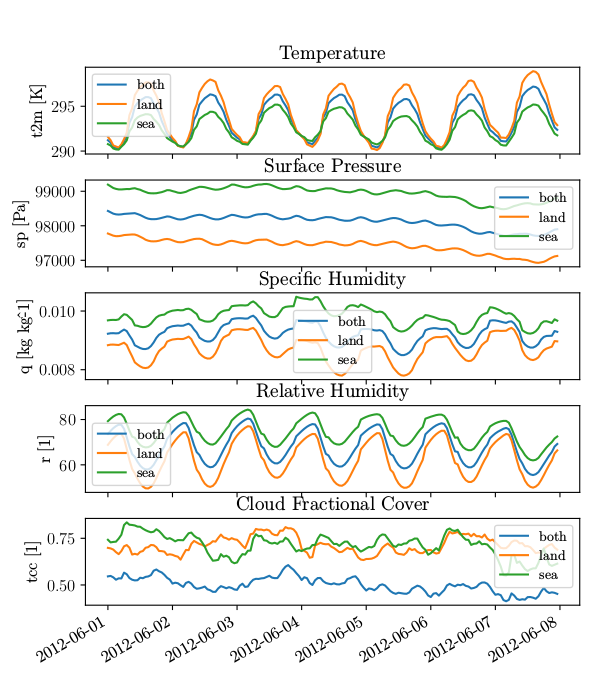
\includegraphics{python_figs/spatially_averaged_one_week_from_2012-06-01.png}
    \caption{Signal June 2012.}
    \label{fig:jun12}
\end{figure}

\begin{figure}[ht]
    \centering
    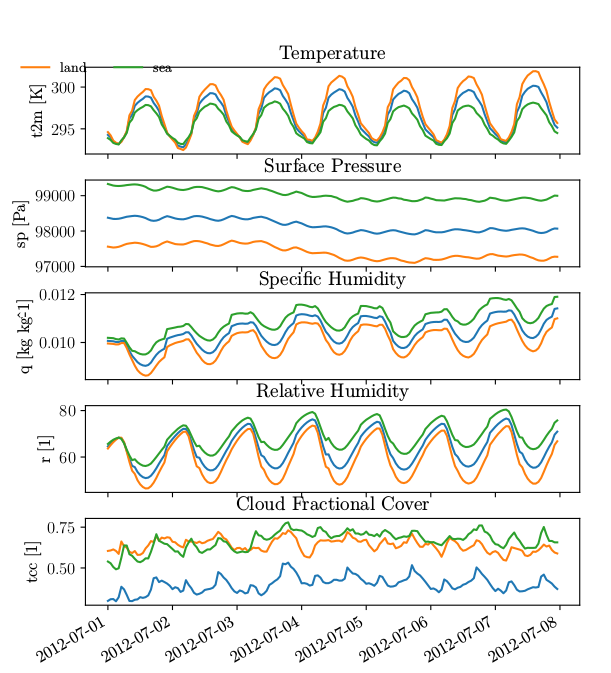
\includegraphics{python_figs/spatially_averaged_one_week_from_2012-07-01.png}
    \caption{Signal July 2012.}
    \label{fig:jul12}
\end{figure}

\begin{figure}[ht]
    \centering
    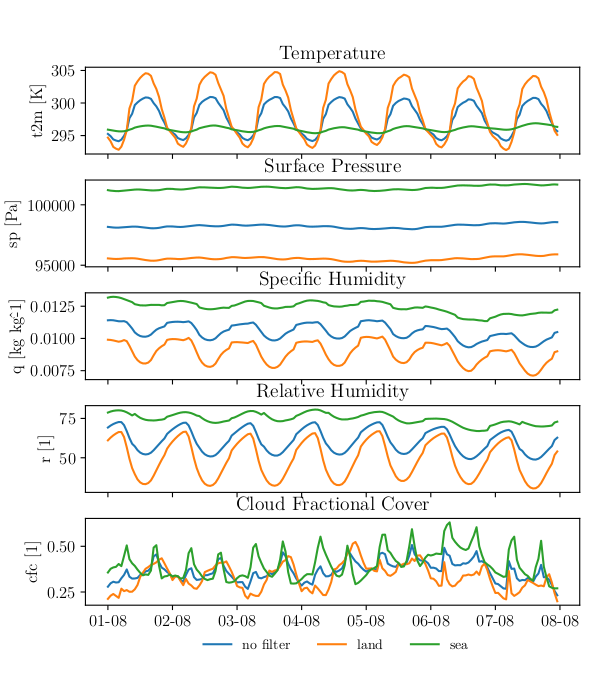
\includegraphics{python_figs/spatially_averaged_one_week_from_2012-08-01.png}
    \caption{Signal August 2012.}
    \label{fig:jan12}
\end{figure}

\begin{figure}[ht]
    \centering
    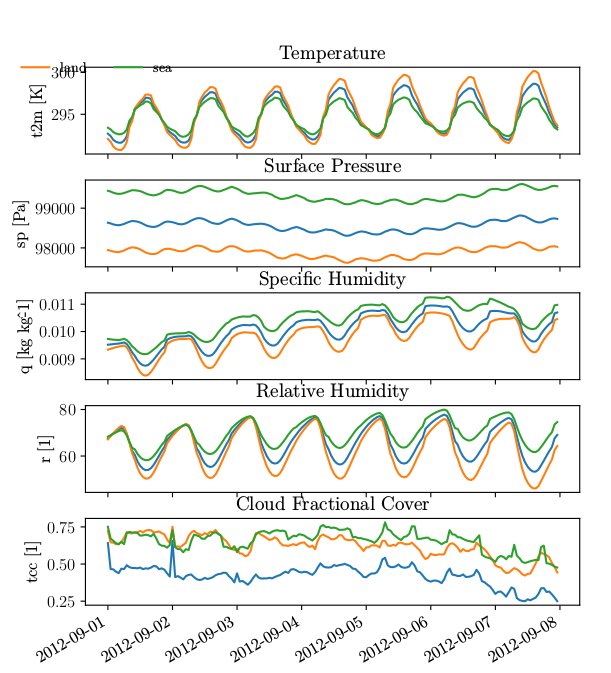
\includegraphics{python_figs/spatially_averaged_one_week_from_2012-09-01.png}
    \caption{Signal September 2012.}
    \label{fig:sep12}
\end{figure}


\begin{figure}[ht]
    \centering
    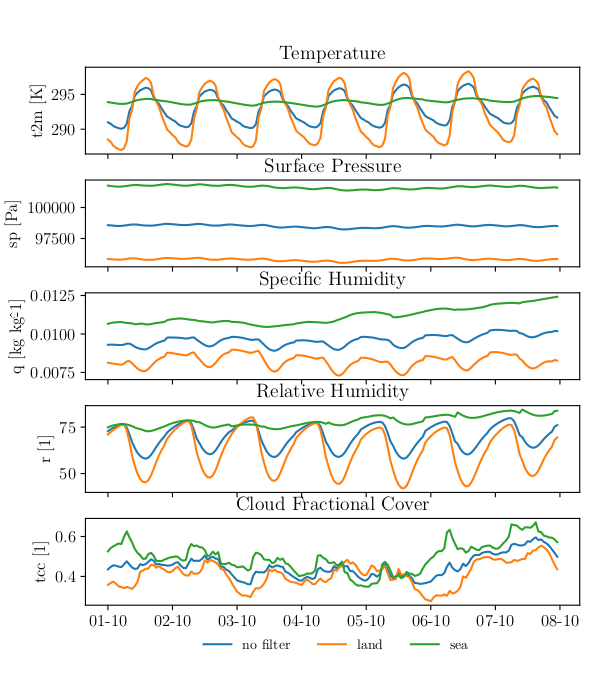
\includegraphics{python_figs/spatially_averaged_one_week_from_2012-10-01.png}
    \caption{Signal October 2012.}
    \label{fig:oct12}
\end{figure}


\begin{figure}[ht]
    \centering
    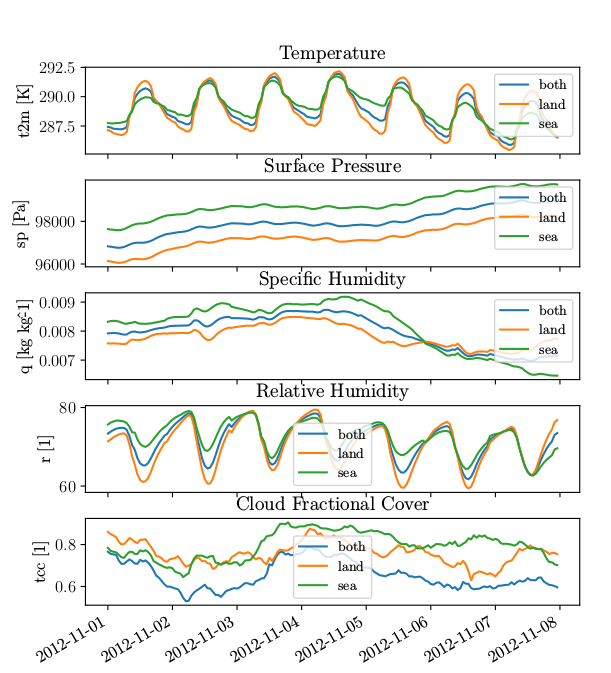
\includegraphics{python_figs/spatially_averaged_one_week_from_2012-11-01.png}
    \caption{Signal November 2012.}
    \label{fig:nov12}
\end{figure}

\begin{figure}[ht]
    \centering
    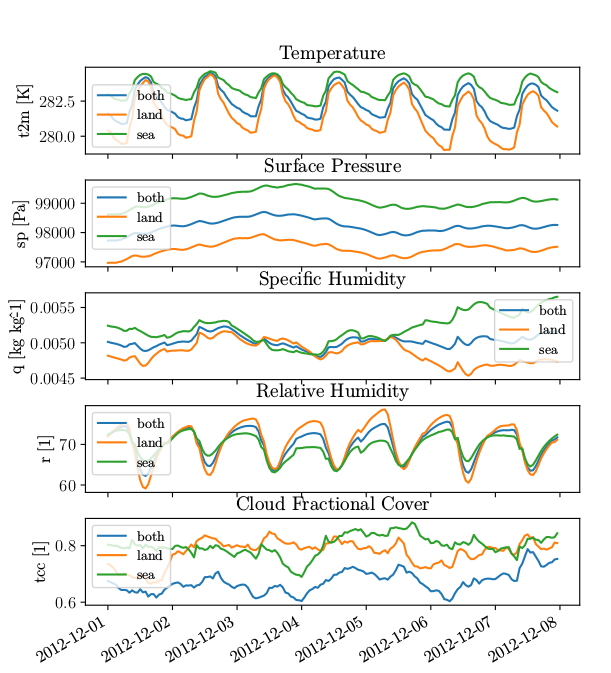
\includegraphics{python_figs/spatially_averaged_one_week_from_2012-12-01.png}
    \caption{Signal December 2012.}
    \label{fig:dec12}
\end{figure}

\chapter{Seasonal effects}
%\addcontentsline{toc}{chapter}{Seasonal effects}
This section has more plots. 
\begin{figure}[ht]
    \centering
    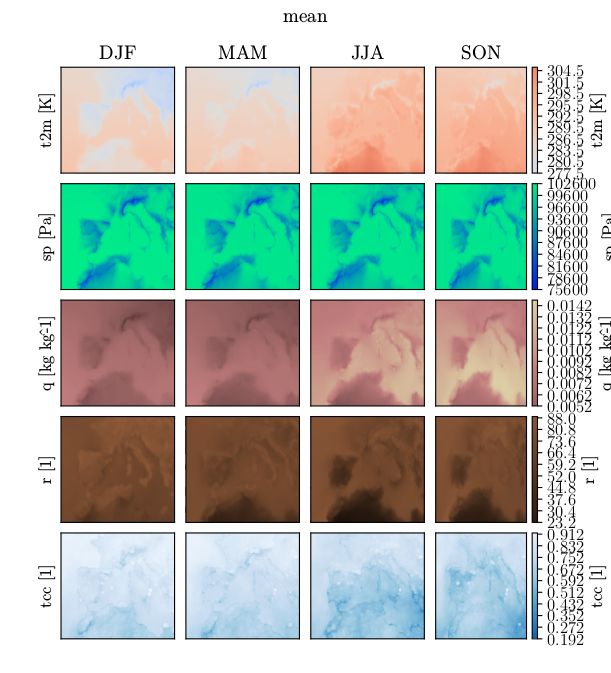
\includegraphics{python_figs/seasonal_mean_all_variables.png}
    \caption{Seasonal mean}
    \label{fig:seasonal_mean}
\end{figure}


\begin{figure}[ht]
    \centering
    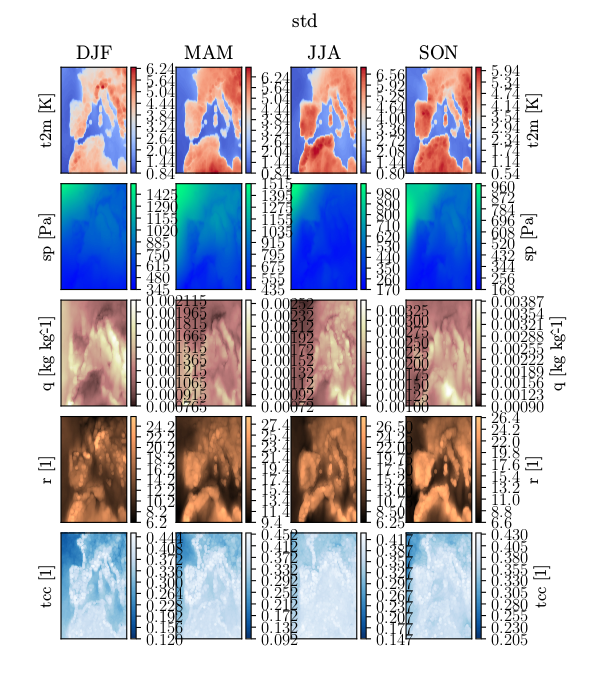
\includegraphics{python_figs/seperate_colorbar_seasonal_std_all_variables.png}
    \caption{Need a colorbar for each plot to study the standard deviation, since the model output has so low std. Seasonal standarddeviation. }
    \label{fig:seasonal_std}
\end{figure}
